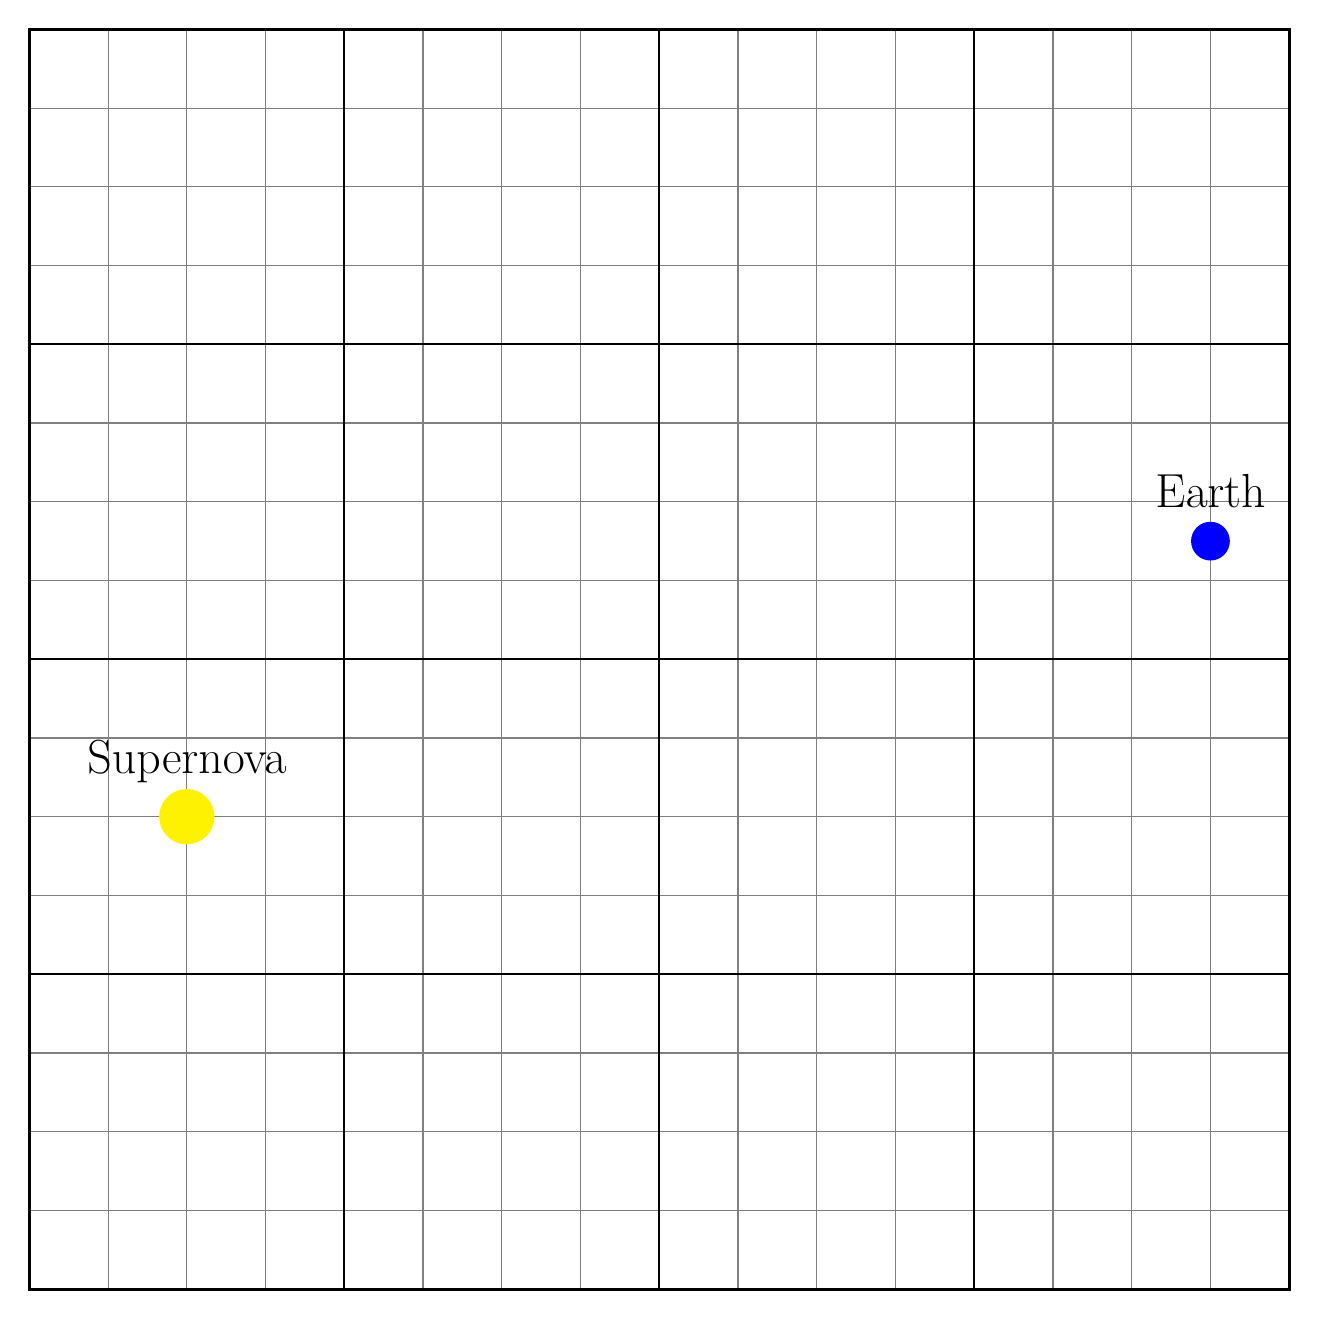
\begin{tikzpicture}[thick,font=\LARGE]
    \draw[step=1cm,gray,thin] (0,0) grid (16,16);
    \draw[step=4cm,black] (0,0) grid (16,16);
    \draw[black,very thick] (0,0) rectangle (16,16);

    \coordinate [label={[label distance=.3cm]above:Supernova}] (S) at (2,6);
    \coordinate [label={[label distance=.3cm]above:Earth}] (E) at (15,9.5);
    \fill [yellow] (S) circle (10pt);
    \fill [blue] (E) circle (7pt);
\end{tikzpicture}

% vim: set ff=unix tw=79 sw=4 ts=4 et ic ai :
